\chapter{Results}
\label{chap:results}

\section{General Information}
\label{sec:general_info}
In total there were 120 participants in the study who made a submission according to Prolific. 12 were removed due to technical issues with the submissions, either their submissions were not received due to technical issues or they actually did not fully complete the experiment. Another 3 were removed due to having missing data in some of the trials and another 4 were removed due to having accuracy on Unambiguous trials below 75\% according to our preregistration \citep{preregistration}. This left us with 101 participants for the analysis. 

It is worth noting that due to the nature of the experiment, the calibration was challenging to pass, making the experiment difficult to complete. 120 participants completed the experiment, however, there were around 150 submission attempts that were not completed. This mainly happened because of the calibration difficulties, according to feedback from some participants. This information gives us an idea about the completion rate of the experiment, which amounted to around 40\%. However, this allowed us to collect a large amount of good quality data, which is the most important aspect of the experiment.

Due to the complexity of the mixed effects models, convergence issues arose. Therefore, the random effects were removed one by one from the models based on the least variance among the random effects. The process was repeated until the models converged. In the case of predicting accuracy, the random effects were removed from the model entirely. 

The general information about the accuracy on the participant level can be seen in \autoref{fig:scatter_acc} and \autoref{fig:hist_acc}. The \autoref{fig:scatter_acc} demonstrates that $L_2$ reasoning takes the largest portion of the participants. This is probably the case due to the included feedback in the trials, which greatly improves the probability of a participant learning a strategy to solve the trials from all 3 conditions. However, generally the data follows similar pattern to the one reported in \cite{Franke_2016}, similar scatter plot can be seen in \autoref{fig:prob_stats}. It is worth to note that a few participants achieved extremely low accuracy on Simple trials, while performing relatively better on Complex trials. The cause of this is unclear.

The histogram in \autoref{fig:hist_acc} shows that the general pattern of people easily solving the Unambiguous trials, struggling more in the Simple condition and finding the Complex condition the most difficult to solve.

\begin{figure}
\centering
\begin{floatrow}
    \ffigbox[\FBwidth]{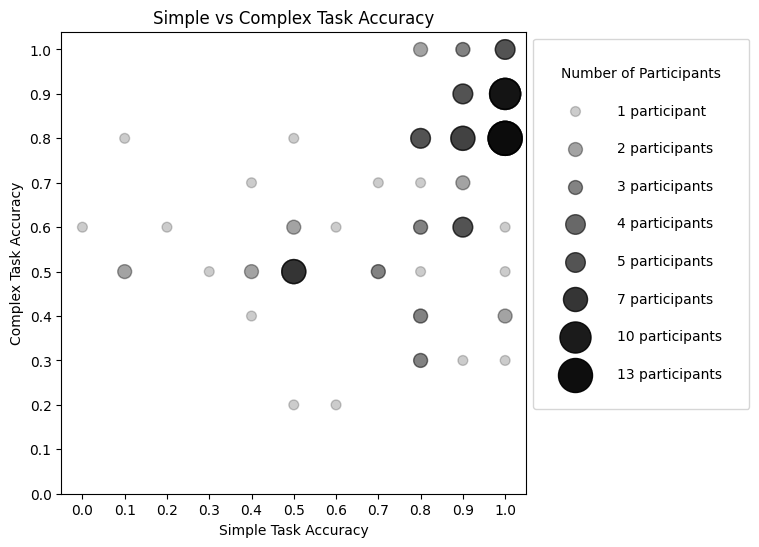
\includegraphics[width=0.55\textwidth]{images/scatter_acc.png}}{
        \caption{Scatter plot of accuracy.}
        \label{fig:scatter_acc}
    }
    \ffigbox[\FBwidth]{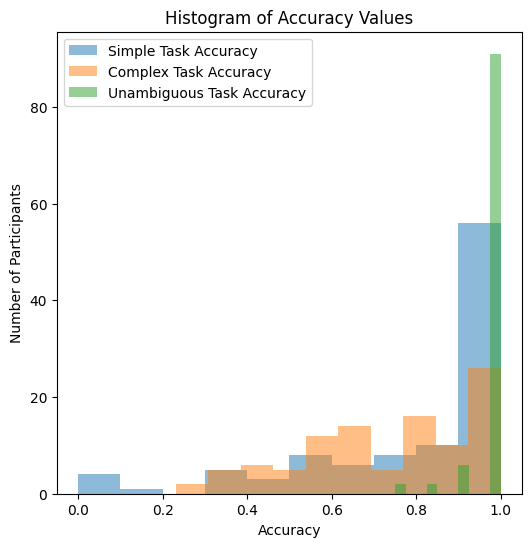
\includegraphics[width=0.385\textwidth]{images/hist_acc.png}}{
        \caption{Histogram of accuracy.}
        \label{fig:hist_acc}
    }
\end{floatrow}
\end{figure}












\section{Pairwise Correlations}
\label{sec:pairwise_corr}

\begin{table}[h!]
\centering
\begin{tabular}{|l|c|c|c|c|}
\hline
\textbf{Feature} & \textbf{Mean (SD)} & \textbf{Accuracy} & \textbf{Mean Answer Time} \\ \hline
PropTimeOnSentMsg & 0.29 (0.09) & -0.33 *** & -0.57 *** \\ \hline
PropTimeOnAvailableMsgs & 0.11 (0.07) & 0.35 *** & 0.38 *** \\ \hline
PropTimeOnTrgt & 0.24 (0.06) & 0.35 *** & 0.18 \\ \hline
PropTimeOnDist & 0.16 (0.06) & -0.03 & 0.29 ** \\ \hline
PropTimeOnComp & 0.18 (0.06) & -0.24 * & -0.07 \\ \hline
PropTimeOnNonAOI & 0.02 (0.01) & -0.02 & 0.04 \\ \hline
RateTogglingAvailableMsgs & 0.04 (0.02) & 0.41 *** & 0.44 *** \\ \hline
NumTogglesAvailableMsgs & 4.39 (3.23) & 0.18 & 0.65 *** \\ \hline
MeanAnswerTime (ms) & 5188 (2586) & 0.08 & --- \\ \hline
Accuracy & 0.8 (0.25) & --- & --- \\ \hline
\end{tabular}
\caption{Simple condition. Correlation table showing the relationships between features, accuracy, and mean answer time. Significance levels: * $p < 0.05$, ** $p < 0.01$, *** $p < 0.001$.}
\label{tab:correlation_table_simple}
\end{table}

The pairwise correlations for the Simple and Complex conditions can be seen in \autoref{tab:correlation_table_simple} and \autoref{tab:correlation_table_complex} correspondingly. The correlations between the eye-tracking features were excluded due to the way they were defined. Almost all of them have negative correlation because the features are proportional and increase in one of them means a decrease in some of the others. However, there was one exception to this general trend, it is a positive significant correlation of 0.2 between the \texttt{PropTimeOnDist} and \texttt{PropTimeOnNonAOI} on Complex condition. This indicates that on Complex trials, the more time a participant spends on the Distractor, the more time they spend outside of the AOI. Generally the Non-AOI feature is extremely low comparing to other eye-tracking features. The only reasonable explanation is that due to the increase in difficulty in the Complex trials, the participants are more likely to have a more of an equally distributed attention across the areas of interest.

Looking at the correlations with accuracy, there are some significant effects. For both conditions, the two less interesting ones are the correlations with \texttt{PropTimeOnTrgt} and \texttt{PropTimeOnComp}. In the former case, there is a significant positive correlation between \texttt{PropTimeOnTrgt} and \texttt{Accuracy}. The more participant look at the Target, the more likely they are to answer correctly. This is not surprising as the Target is the correct answer. A similar logic can be applied to the later, there is a significant negative correlation between \texttt{PropTimeOnComp} and \texttt{Accuracy}. The more time a participant spends looking at the Competitor, the more likely they are to choose it, therefore, answering incorrectly. In addition, we visually inspected the scanpaths of some participants. The effect might be coming from the last look at the object of choice, therefore, tipping the proportional time in favor of the chosen object and, hence, correlating the proportional time to the answer.

\begin{table}[h!]
\centering
\begin{tabular}{|l|c|c|c|c|}
\hline
\textbf{Feature} & \textbf{Mean (SD)} & \textbf{Accuracy} & \textbf{Mean Answer Time} \\ \hline
PropTimeOnSentMsg & 0.26 (0.09) & -0.35 *** & -0.61 *** \\ \hline
PropTimeOnAvailableMsgs & 0.13 (0.07) & 0.22 * & 0.51 *** \\ \hline
PropTimeOnTrgt & 0.23 (0.07) & 0.56 *** & 0.02 \\ \hline
PropTimeOnDist & 0.15 (0.06) & -0.08 & 0.19 \\ \hline
PropTimeOnComp & 0.21 (0.06) & -0.26 ** & 0.11 \\ \hline
PropTimeOnNonAOI & 0.02 (0.02) & -0.01 & 0.01 \\ \hline
RateTogglingAvailableMsgs & 0.04 (0.02) & 0.25 * & 0.45 *** \\ \hline
NumTogglesAvailableMsgs & 5.19 (3.69) & 0.23 * & 0.78 *** \\ \hline
MeanAnswerTime (ms) & 6565 (4022) & 0.18 & --- \\ \hline
Accuracy & 0.7 (0.21) & --- & --- \\ \hline
\end{tabular}
\caption{Complex condition. Correlation table showing the relationships between features, accuracy, and mean answer time. Significance levels: * $p < 0.05$, ** $p < 0.01$, *** $p < 0.001$.}
\label{tab:correlation_table_complex}
\end{table}

Furthermore, the \texttt{PropTimeOnSentMsg} has a significant negative correlation with accuracy in both conditions. This indicates that the more time a participant spends looking at the sent message, the less likely they are to answer correctly. This can be explained by the fact that the sent message is important in the trial, however, spending more time looking at it would mean that less time is spent looking at the other crucial areas of interest. And a better accuracy is achieved probably by taking a quick look at the sent message and then focusing on the other areas of interest. 

As for the \texttt{PropTimeOnAvailableMsgs}, it has a significant positive correlation with accuracy in both conditions. This indicates that the more time a participant spends looking at the available messages, the more likely they are to answer correctly. This is not surprising as the available messages are extremely important to solve the Simple trials. It is worth noting that the effect is much stronger in the Simple condition, where the correlation is 0.35, comparing to the Complex condition, where the correlation is 0.22. This partially aligns with the second hypothesis described in \autoref{sec:h2}. The effect is significant in both conditions. While we anticipated that the Simple condition would benefit from the available messages more, the Complex condition also benefits from it. This is probably due to the fact that the available messages are still important for the participants in the Complex trials.

Both \texttt{RateTogglingAvailableMsgs} and \texttt{NumTogglesAvailableMsgs} show significant positive correlations with accuracy in Complex condition. However, in simple condition, only the \texttt{RateTogglingAvailableMsgs} shows a significant positive correlation with accuracy. This indicates that the raw amount of toggles is not important by itself, but only shows up as significant when combined with answer time. Potentially indicating that a certain successful strategy is encoded in the high rate of toggling for Simple trials.

\sloppy
Now, looking at the column of \texttt{MeanAnswerTime}. We did not make any hypothesis about how answer time would relate to the eye-tracking features, however, it can still give us some general information about participant-level patterns. The \texttt{PropTimeOnSentMsg} has a significant negative correlation with the answer time. The reason for this is probably related to the interpretation of the correlation with the accuracy. Participants might adapt a suboptimal strategy where they would not look at the available messages which works perfectly for the Unambiguous trials, however, completely fails on the Simple trials. That is why the proportional increase in time spent looking at the sent message indicates a quick answer and low accuracy. 
\sloppy

The \texttt{PropTimeOnAvailableMsgs} has a significant positive correlation with the answer time. This indicates that the more time a participant spends looking at the available messages, the more time they would spend on the trial in general. This is not surprising as proportionally spending more time looking at the available messages indicates more reasoning involved in the problem solving process, which leads to more time spent on the trial. Especially taking into account the fact that the available messages has second to lowest average time spent on it in both conditions. 

\texttt{NumTogglesAvailableMsgs} have significant positive correlations with the answer time in both conditions. This is expected as the raw number of toggles increases with time spent on trial. On the other hand, a positive significant correlation of \texttt{RateTogglingAvailableMsgs} with the answer time in both conditions indicates that the more time is spent on the trial, the more participants tend to toggle. 

Last but not least is the \texttt{PropTimeOnDist}. It has a significant positive correlation with the answer time only in the Simple trials. This indicates that the more time a participant spends looking at the Distractor, the more time they would spend on the trial in general. This is not surprising as the Distractor is not an important feature in the Simple trials, however, spending more time looking at it would mean that less time is spent looking at the other crucial areas of interest.

\sloppy
The pairwise correlations for the Unambiguous condition were not included in the tables because there were very few significant effects. There were no significant correlations with accuracy, however, the \texttt{PropTimeOnComp}, \texttt{PropTimeOnDist} and \texttt{PropTimeOnAvailableMsgs} have significant positive correlations with the answer time. This is because the Unambiguous trials are very easy to solve, therefore, the participants do not need to look at the Distractor, Competitor or available messages at all. The only feature that has a significant negative correlation with the answer time is \texttt{PropTimeOnSentMsg}. This is not surprising as the sent message is perhaps the most important feature in the Unambiguous trials. A more detailed explanation and the table can be found in \autoref{sec:pairwise_corr_unambiguous}.
\sloppy

\subsection*{Conclusion}
The pairwise correlations gave us some general understanding about which features are important. The most important finding is, the significant correlation of \texttt{PropTimeOnAvailableMsgs} and \texttt{RateTogglingAvailableMsgs} to the accuracy in both Simple and Complex conditions. As well as the absence of significant correlation between the \texttt{PropTimeOnDist} and accuracy. This hints us that participants look similarly on the trial in terms of proportional time, but still achieve different accuracy. From here we will move to the linear regression predicting accuracy. 















\section{Predicting Accuracy}
\label{sec:accuracy_model}

The final formula for the model predicting accuracy is presented below. All random effects were removed from the model due to convergence issues:
\begin{verbatim}
    Correct ~ Condition + TrgtPos + Trial +
    PropTimeOnTrgt + PropTimeOnComp + PropTimeOnDist +
    PropTimeOnSentMsg + PropTimeOnAvailableMsgs +
    RateTogglingAvailableMsgs + MsgType + AnswerTime +
    Condition:PropTimeOnTrgt + Condition:PropTimeOnComp +
    Condition:PropTimeOnDist + Condition:PropTimeOnSentMsg +
    Condition:PropTimeOnAvailableMsgs +
    Condition:RateTogglingAvailableMsgs +
    Condition:AnswerTime +
    (1 + Condition + TrgtPos + Trial + PropTimeOnTrgt +
    PropTimeOnComp + PropTimeOnDist + PropTimeOnSentMsg +
    PropTimeOnAvailableMsgs + RateTogglingAvailableMsgs +
    MsgType | Subject) 

\end{verbatim}
The model had the following encodings for the categorical variables \autoref{tab:msgtype_encoding}, \autoref{tab:trgtpos_encoding} and \autoref{tab:condition_encoding}. The Target position can be interpreted as comparing left to center or right and right to center or left for features ``TrgtPos2'' and ``TrgtPos3'' respectively. The condition can be interpreted as comparing the Simple condition to the Complex condition and the Unambiguous condition to the Simple and Complex conditions together. The model was trained using the \texttt{lme4} package in R. The model was trained using the \texttt{glm} function with the following parameters: \texttt{family = binomial(link = "logit")}. The resulting coefficients can be seen in \autoref{tab:model_coefficients_acc}. 

\begin{table}[h!]
    \centering
    \begin{tabular}{|c|c|}
    \hline
    Message Type & MsgType \\ \hline
    Shape        & -1       \\ \hline
    Color        & 1        \\ \hline
    \end{tabular}
    \caption{Encoding of the message type categorical variable.}
    \label{tab:msgtype_encoding}
    \end{table}
    \hfill
    \begin{table}[h!]
    \centering
    \begin{tabular}{|c|c|c|c|}
    \hline
    Target Position & TrgtPos2 & TrgtPos3\\ \hline
    0               & 1    & 0    \\ \hline
    1               & 0    & 0    \\ \hline
    2               & 0    & 1    \\ \hline
    \end{tabular}
    \caption{Encoding of the Target position categorical variable.}
    \label{tab:trgtpos_encoding}
    \end{table}
    \begin{table}[h!]
    \centering
    \begin{tabular}{|c|c|c|}
    \hline
    Condition     & Condition1 & Condition2 \\ \hline
    Complex       & -1   & -1   \\ \hline
    Simple        & 1    & -1   \\ \hline
    Unambiguous   & 0    & 2    \\ \hline
    \end{tabular}
    \caption{Encoding of the condition categorical variable.}
    \label{tab:condition_encoding}
\end{table}


Looking at some general findings from \autoref{tab:model_coefficients_acc}, starting from the Intercept, it is positive and significant, indicating that having no information about any of the features, the trial is more likely to be solved correctly. This is unsurprising as the average accuracy across all trials amounted to 82.5\%. 

One can see from \texttt{Condition1} that the Complex trials are predicted to have significantly lower accuracy comparing to the Simple ones. However, the effect is not fully captured by this coefficient due to the inclusion of the interaction terms. \texttt{Condition2} indicates that Unambiguous trials have a higher probability of being solved correctly comparing to Simple and Complex ones, the effect is also significant. So far, the findings fully align with how the trials were designed. 

\texttt{TrgtPos2} and \texttt{TrgtPos3} effects are harder to interpret. The findings suggest that the when the Target is on the left or right side, the probability of correctly answering increases, the effect is significant. This might be somehow related to the fact that the objects are split far apart from each other.

\begin{table}[h!]
\centering
\begin{tabular}{|l|c|c|c|c|}
\hline
\textbf{Predictor} & \textbf{Estimate} & \textbf{Std. Error} & \textbf{z value} & \textbf{Pr(>|z|)} \\ \hline
(Intercept)                          & 1.23265 & 0.18460 & 6.677 & 2.43e-11 *** \\ \hline
Condition1                           & 0.22087 & 0.05499 & 4.017 & 5.91e-05 *** \\ \hline
Condition2                           & 1.10938 & 0.14302 & 7.757 & 8.69e-15 *** \\ \hline
TrgtPos2                             & 1.92305 & 0.21183 & 9.078 & < 2e-16 *** \\ \hline
TrgtPos3                             & 1.69844 & 0.20450 & 8.305 & < 2e-16 *** \\ \hline
Trial                                & 0.22635 & 0.04825 & 4.691 & 2.72e-06 *** \\ \hline
PropTimeOnTrgt                      & -6.09992 & 6.15675 & -0.991 & 0.3218 \\ \hline
PropTimeOnComp                     & -12.92581 & 6.16769 & -2.096 & 0.0361 * \\ \hline
PropTimeOnDist                     & -11.95582 & 6.14733 & -1.945 & 0.0518 . \\ \hline
PropTimeOnSentMsg                   & -9.95567 & 6.06806 & -1.641 & 0.1009 \\ \hline
PropTimeOnAvailableMsgs             & -8.69726 & 6.27784 & -1.385 & 0.1659 \\ \hline
MsgType                            & -0.11506 & 0.04888 & -2.354 & 0.0186 * \\ \hline
AnswerTime                          & -0.12537 & 0.05186 & -2.418 & 0.0156 * \\ \hline
Condition1:PropTimeOnTrgt           & -1.93730 & 1.09696 & -1.766 & 0.0774 . \\ \hline
Condition2:PropTimeOnTrgt          & -12.13074 & 6.12982 & -1.979 & 0.0478 * \\ \hline
Condition1:PropTimeOnComp           & -1.30711 & 1.08177 & -1.208 & 0.2269 \\ \hline
Condition2:PropTimeOnComp          & -11.30869 & 6.12510 & -1.846 & 0.0649 . \\ \hline
Condition1:PropTimeOnDist           & -1.13168 & 1.08619 & -1.042 & 0.2975 \\ \hline
Condition2:PropTimeOnDist          & -12.16270 & 6.10435 & -1.992 & 0.0463 * \\ \hline
Condition1:PropTimeOnSentMsg        & -0.97657 & 1.09161 & -0.895 & 0.3710 \\ \hline
Condition2:PropTimeOnSentMsg       & -10.26290 & 6.03306 & -1.701 & 0.0889 . \\ \hline
Condition1:PropTimeOnAvMsgs   & 0.70963 & 1.13710 & 0.624 & 0.5326 \\ \hline
Condition2:PropTimeOnAvMsgs & -12.08512 & 6.24131 & -1.936 & 0.0528 . \\ \hline
Condition1:AnswerTime               & -0.11566 & 0.05769 & -2.005 & 0.0450 * \\ \hline
Condition2:AnswerTime               & -0.02166 & 0.03973 & -0.545 & 0.5856 \\ \hline
\end{tabular}
\caption{Summary of the trained model coefficients. Significance levels: . $p < 0.1$, * $p < 0.05$, ** $p < 0.01$, *** $p < 0.001$.}
\label{tab:model_coefficients_acc}
\end{table}

Due to the convergence issues, a corresponding Bayesian model was trained that included all random effects. 




The coefficient for \texttt{Trial} suggests that people get better as they progress through the experiment. This is expected as the participants have feedback after they answer, which tells whether their answer is correct or not. This finding also aligns with some of the findings from the previous work \citep{Mayn_2023, Mayn_2025}. 

Moving to the eye-tracking features, the \texttt{PropTimeOnComp} has a significant negative effect, indicating that the more participants looks at the Competitor, the more likely they are to answer incorrectly. This effect probably comes from the last look that people do before selecting the object which tips the proportional feature. If a participant cannot derive the correct answer through the reasoning, they will most likely guess among the Target and the Competitor as they both share the sent message feature, making looking at the Competitor negatively correlated to the accuracy.

Furthermore, the \texttt{PropTimeOnDist} has a large negative effect, it is almost significant. The effect is most likely coming from the Unambiguous trials which we will discuss later more in details. 

The \texttt{MsgType} indicates that trials where the sent message is a shape are more likely to be solved correctly. The effect is significant, although relatively small.

Regarding the \texttt{AnswerTime}, the general term suggests that the longer one stays on the trial, the more likely they are to answer incorrectly. However, this term should be interpreted together with the interaction terms. We will discuss it further in more details.


\begin{table}[h!]
\centering
\begin{tabular}{|c|c|c|c|c|}
\hline
\textbf{Condition} & \textbf{PropTimeOnDist.trend} & \textbf{SE} & \textbf{asymp.LCL} & \textbf{asymp.UCL} \\ \hline
Complex            & 1.339                        & 1.46        & -1.53              & 4.204              \\ \hline
Simple             & -0.925                       & 1.63        & -4.11              & 2.265              \\ \hline
Unambiguous        & -36.281                      & 18.30       & -72.13             & -0.434             \\ \hline
\end{tabular}
\caption{Trends for proportional time on Distractor based on condition.}
\label{tab:proptimeondist_trends}
\end{table}

\begin{figure}
    \centering
    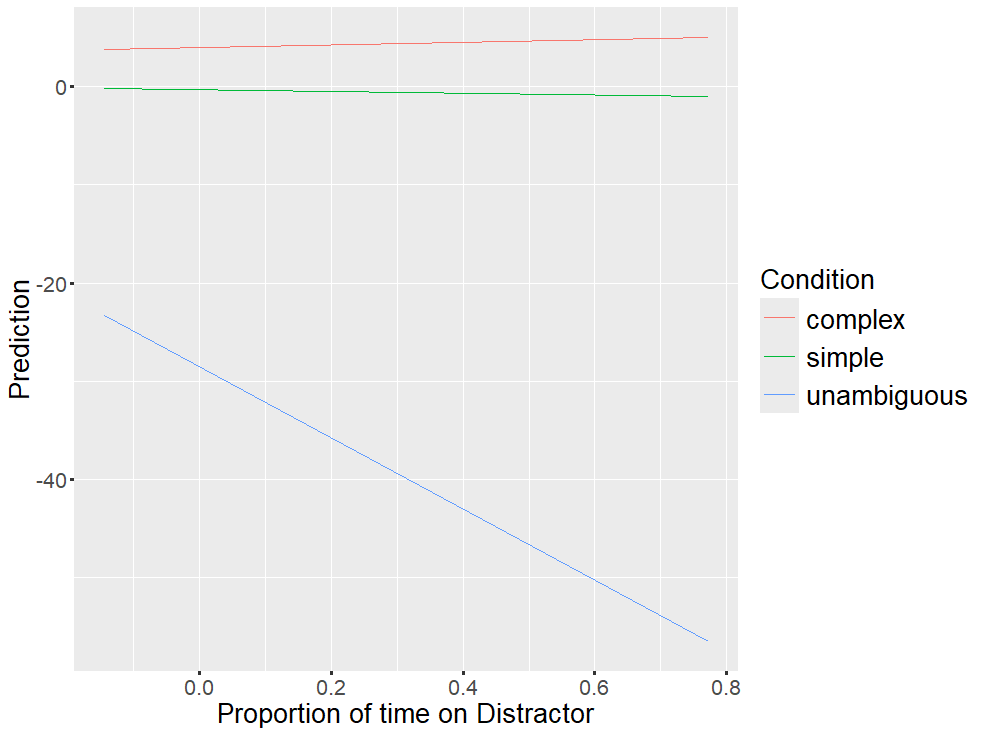
\includegraphics[width=0.8\textwidth]{images/proptimeondist_trends.png}
    \caption{Visualization of trends for proportional time on Distractor based on condition.}
    \label{fig:proptimeondist_trends}
\end{figure}

\begin{table}[h!]
\centering
\begin{tabular}{|c|c|c|c|c|c|}
\hline
\textbf{Contrast} & \textbf{Estimate} & \textbf{SE} & \textbf{z.ratio} & \textbf{p.value} \\ \hline
Complex - Simple & 2.26 & 2.17 & 1.042 & 0.5504 \\ \hline
Complex - Unambiguous & 37.62 & 18.30 & 2.051 & 0.1003 \\ \hline
Simple - Unambiguous & 35.36 & 18.30 & 1.927 & 0.1311 \\ \hline
\end{tabular}
\caption{Contrasts for proportional time on Distractor based on condition.}
\label{tab:proptimeondist_contrasts}
\end{table}

The first hypothesis we were interested in was that proportional time on Distractor is positively associated with accuracy on Complex trials, described in \autoref{sec:h1}. Even though the coefficient for the interaction term ``Condition1:PropTimeOnDist'' is not significant, due to how interaction terms work, we can still interpret how model prediction changes based on the value of the interaction term. First of all, we can take a look at \autoref{tab:proptimeondist_trends} which shows the trends of the Proportional time on Distractor for each condition. As well as the plot \autoref{fig:proptimeondist_trends} which visualizes the trends of the proportional time on Distractor for each condition. The \autoref{tab:proptimeondist_trends} indicates the trends we anticipated, however, the columns \texttt{asymp.LCL} and \texttt{asymp.UCL} indicate the asymptotic lower and upper confidence limits -- that is, the 95\% confidence interval around the slope estimate. In Simple and Complex cases the interval includes 0, making the slopes not significant. It is worth noting that the slope for the Unambiguous trials is very large and ends up as significant in the end. However, the main issue is that the amount of incorrectly solved Unambiguous trials is extremely low, as the average accuracy on Unambiguous trials amounted to 98\%. This fact makes the slope have very large standard error and subsequently the confidence interval is also very spread. To address the potential that the high uncertainty in the Unambiguous conditions affected model fit and quality, we also fit models to only critical conditions, that is only Simple and Complex ones. Convergence difficulties were found to the same degree, and final model estimates for the trends were comparable, with no changes in significance. We continue with the conclusions we drew from the larger model.
Furthermore, we can look at \autoref{tab:proptimeondist_contrasts}. The table indicates the differences between the slopes and gives corresponding p values for them. The row corresponding to our hypothesis is the first one ``Complex - Simple''. the findings indicate that the Complex trials will benefit more from the proportional time on Distractor than the Simple ones. However, again, the effect is not significant. In addition, the estimates for the contrasts that include Unambiguous trials are close to being significant, however, these estimates are likely unreliable due to the reasons we discussed earlier.

\begin{table}[h!]
\centering
\begin{tabular}{|c|c|c|c|c|}
\hline
\textbf{Condition} & \textbf{PropTimeOnAvMsgs.trend} & \textbf{SE} & \textbf{asymp.LCL} & \textbf{asymp.UCL} \\ \hline
Complex            & 2.68                                  & 1.51        & -0.281             & 5.64              \\ \hline
Simple             & 4.10                                  & 1.70        & 0.761              & 7.43              \\ \hline
Unambiguous        & -32.87                                & 18.70       & -69.502            & 3.77              \\ \hline
\end{tabular}
\caption{Trends for proportional time on available messages based on condition.}
\label{tab:proptimeonavmsgs_trends}
\end{table}

The second hypothesis goes as follows, proportional time on available messages is positively associated with accuracy on Simple trials, described in \autoref{sec:h2}. Similarly to how we interpreted the findings for the first hypothesis, we will look at the actual predictions of the model and not solely at the coefficients to capture the whole relation between the interaction terms and the regular ones. The trends are presented in \autoref{tab:proptimeonavmsgs_trends}. From the table we can indeed see a positive effect of proportional time on available messages on Simple condition. Therefore, the findings support the second hypothesis. In addition, the confidence interval does not include 0, suggesting that the effect is significant. As for the Complex and Unambiguous trials, neither of the effects are significant, however, the trend for the Complex trial is also positive, suggesting that the available messages are still important for the participants in the Complex trials. It is worth noting, that the Complex trials can be solved without knowing the available messages at all as was described in \autoref{sec:h2}. Hence, the available messages might not be as important in the Complex condition.


Taking into account the fact that \texttt{AnswerTime} and one of the interaction terms including it have significant effects, we will also interpret the trends for this feature.  The trends can be seen in \autoref{tab:answertime_trends}. From the table we can conclude that the answer time on the Simple condition has a significant negative effect. This means, that the longer one takes to solve the Simple case, the more likely they are to answer incorrectly. The slopes for the other conditions are not significant.

\begin{table}[h!]
\centering
\begin{tabular}{|c|c|c|c|c|}
\hline
\textbf{Condition} & \textbf{AnswerTime.trend} & \textbf{SE} & \textbf{asymp.LCL} & \textbf{asymp.UCL} \\ \hline
Complex            & 0.012                     & 0.0678      & -0.121             & 0.1449             \\ \hline
Simple             & -0.219                    & 0.0938      & -0.403             & -0.0356            \\ \hline
Unambiguous        & -0.169                    & 0.1040      & -0.372             & 0.0351             \\ \hline
\end{tabular}
\caption{Trends for Answer Time based on condition.}
\label{tab:answertime_trends}
\end{table}




\begin{table}[ht]

\centering
\caption{Bayesian logistic regression coefficients. All \(\hat{R}\) values were equal to 1, indicating convergence.}
\begin{tabular}{lrrrr}
\hline
\textbf{Predictor} & \textbf{Estimate} & \textbf{Est. Error} & \textbf{2.5\% CI} & \textbf{97.5\% CI} \\
\hline
Intercept                                & 0.74 & 0.25 & 0.26 & 1.25 \\
Condition1                               & 0.57 & 0.12 & 0.34 & 0.82 \\
TrgtPos2                                 & 2.21 & 0.33 & 1.58 & 2.88 \\
TrgtPos3                                 & 1.94 & 0.32 & 1.34 & 2.59 \\
Trial                                    & 0.45 & 0.09 & 0.28 & 0.64 \\
PropTimeOnTrgt                           & 6.52 & 1.41 & 3.77 & 9.29 \\
PropTimeOnComp                          & -2.50 & 1.29 & -5.06 & -0.00 \\
PropTimeOnDist                           & 0.21 & 1.29 & -2.33 & 2.71 \\
PropTimeOnSentMsg                        & 0.84 & 1.30 & -1.71 & 3.37 \\
PropTimeOnAvailableMsgs                  & 2.74 & 1.40 & -0.01 & 5.46 \\
RateTogglingAvailableMsgs                & 1.64 & 2.35 & -2.86 & 6.29 \\
MsgType1                                & -0.17 & 0.09 & -0.35 & 0.00 \\
AnswerTime                              & -0.20 & 0.09 & -0.37 & -0.03 \\
Condition1:PropTimeOnTrgt               & -2.59 & 1.27 & -5.08 & -0.12 \\
Condition1:PropTimeOnComp               & -1.81 & 1.26 & -4.31 & 0.64 \\
Condition1:PropTimeOnDist               & -1.43 & 1.26 & -3.91 & 1.03 \\
Condition1:PropTimeOnSentMsg            & -1.08 & 1.27 & -3.61 & 1.36 \\
Condition1:PropTimeOnAvailableMsgs      & -0.52 & 1.37 & -3.25 & 2.15 \\
Condition1:RateTogglingAvailableMsgs     & 4.24 & 2.29 & -0.21 & 8.70 \\
Condition1:AnswerTime                   & -0.12 & 0.08 & -0.28 & 0.04 \\
\hline
\end{tabular}
\label{tab:bayesian_model_coefficients_acc}
\end{table}

\emph{The decomposition by condition was observed similarly to the MLE model. However, in the case of Bayesian model, none of the interesting effects were found to be significant. }



\subsection{LASSO Regression}
\label{sec:lasso_regression}
In order to further understand the importance of the features, we trained a LASSO regression model on the same data. The model was trained using the \texttt{glmnet} package in R. The model was trained using the \texttt{cv.glmnet} function with LOOCV (Leave-One-Out Cross-Validation) on participant level, the data, on the other hand is at trial level. The model was trained with the following parameters: \texttt{alpha = 1, family = "binomial", foldid = as.numeric(data\$Subject)}. We proceed to visualize the LASSOO results with the following plot \autoref{fig:lasso_plot}.

\begin{figure}[h!]
    \centering
    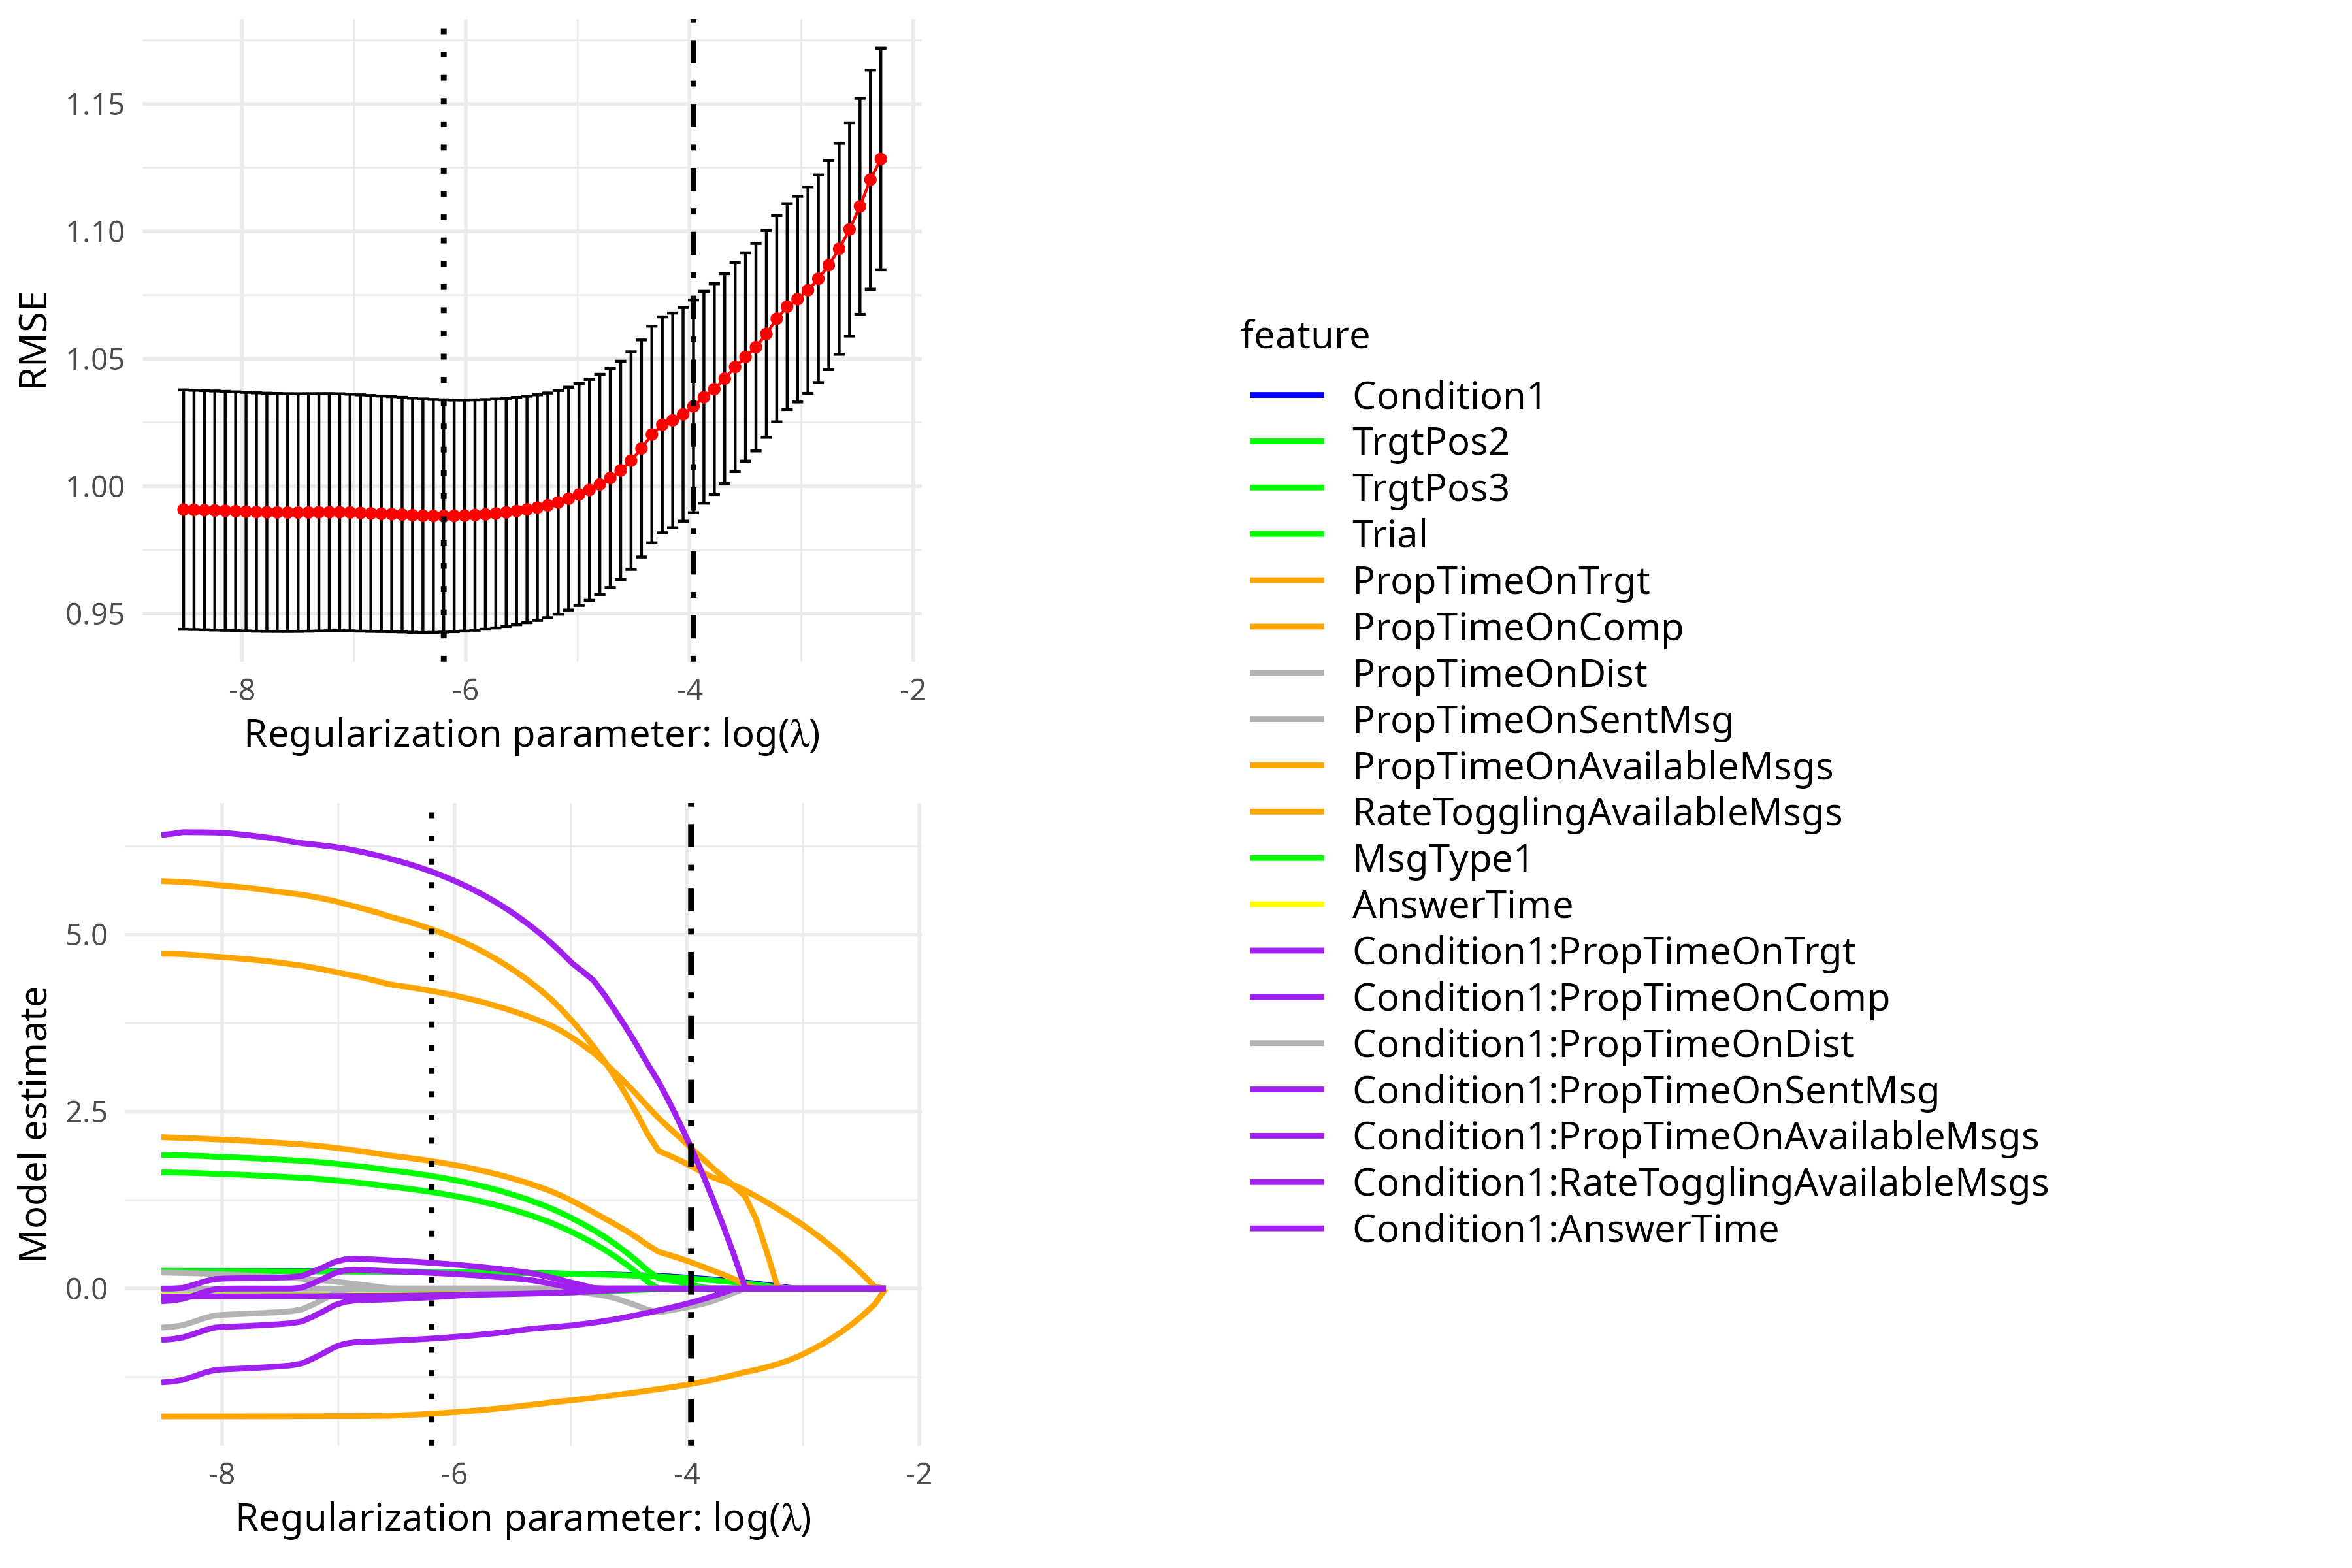
\includegraphics[width=0.8\textwidth]{images/lasso_plot_correct.png}
    \caption{LASSO regression coefficients.}
    \label{fig:lasso_plot}
\end{figure}

\TODO{Right something about the LASSO regression results.}



\subsection*{Conclusion}
The first hypothesis with the Distractor was not confirmed by the main model. That is, the proportional time on Distractor is not positively associated with the accuracy on Complex trials. On the other hand, the proportional time on available messages is significantly positively associated with the accuracy on Simple trials. 

The full conclusion will be drawn later, however, the general pattern suggests that participants fail to solve the trial not due to the lack of information, but rather due to lack of depth during the reasoning process. While the proportional time on available messages might to some extent describe the reasoning process.
















\section{On Distractor}
\label{sec:distractor_model}

The model presented here predicts the likelihood (binary outcome) of participants gazing at the Distractor during correctly solved trials. The final formula for the model predicting the likelihood of looking at the Distractor for the correctly solved trials is presented below. Most of the random effects were removed from the model due to convergence issues:
\begin{verbatim}
    OnDist ~ Condition + Trial + MsgType + TrgtPos +
        (1 | Subject)
\end{verbatim}

\begin{table}[h!]
\centering
\begin{tabular}{|l|c|c|c|c|}
\hline
\textbf{Coefficient} & \textbf{Estimate} & \textbf{Std. Error} & \textbf{z value} & \textbf{Pr(>|z|)} \\ \hline
(Intercept)          & -3.056241         & 0.039379            & -77.611          & <2e-16 ***        \\ \hline
Condition1           & 0.013373          & 0.006440            & 2.076            & 0.0379 *          \\ \hline
Condition2           & -0.086425         & 0.004691            & -18.425          & <2e-16 ***        \\ \hline
Trial                & -0.053649         & 0.005713            & -9.391           & <2e-16 ***        \\ \hline
MsgType             & -0.017492         & 0.005713            & -3.062           & 0.0022 **         \\ \hline
TrgtPos2             & 1.772965          & 0.018094            & 97.986           & <2e-16 ***        \\ \hline
TrgtPos3             & 1.795716          & 0.018151            & 98.931           & <2e-16 ***        \\ \hline
\end{tabular}
\caption{Summary of the model predicting the likelihood of looking at the Distractor for the correctly solved trials. Significance levels: * $p < 0.05$, ** $p < 0.01$, *** $p < 0.001$.}
\label{tab:model_coefficients_distractor}
\end{table}

In this case, no interaction terms were included in the model. Hence, the model coefficients can be interpreted directly as each coefficient is the effect of the corresponding feature that appears only once in the whole model. The encodings for the categorical variables are the same as in \autoref{tab:msgtype_encoding}, \autoref{tab:trgtpos_encoding} and \autoref{tab:condition_encoding}. The model was trained using the \texttt{lme4} package in R. The model was trained using the \texttt{glmer} function with the following parameters: \texttt{family = binomial(link = "logit")}. The resulting coefficients can be seen in \autoref{tab:model_coefficients_distractor}.

Starting from the Intercept, it is negative and significant, indicating that without any information about the correctly solved trial, the predicted gaze point is likely to be not on the Distractor. This is unsurprising as the average time spent looking at the Distractor was 14.3\% across all correctly solved trials. 

\texttt{Condition1} indicates that the Distractor is more likely to be looked at in the Simple trials than in the Complex ones. This finding is the opposite of what we expected according to the hypothesis 3 described in \autoref{sec:h3}. The effect is small but significant. This indicates that taking into account the correctly solved trials, not only the Distractor was not looked at more in the Complex trials, but it was actually looked at more in the Simple trials. A possible explanation is that a skilled participant would apply the same strategy to both the Simple and Complex trials. \texttt{Condition2} indicates that the Distractor is less likely to be looked at in the Unambiguous trials than in the Simple and Complex ones. The effect is significant and large, indicating that the Distractor is not looked at as much in the Unambiguous trials. This finding is not surprising as the Distractor is not important in the Unambiguous trials. More importantly this implies that skilled participants tend to use different strategies in Unambiguous trials comparing to Simple and Complex ones.

\texttt{Trial} indicates that the Distractor is less likely to be looked at as the trial number increases. This is expected as the participants get more efficient as they progress through the experiment. While closer to the beginning they would explore the trials more thoroughly, later on they would be more likely to look at other areas of interest and not at the Distractor, which is not as important. 

\texttt{MsgType} indicates that the Distractor is less likely to be looked at when the sent message is a color. The effect is significant but relatively small. We were unable to find a reasonable explanation for this effect.

\texttt{TrgtPos2} and \texttt{TrgtPos3} indicate that the Distractor is more likely to be looked at when the Target is on the left or right side. The effect is significant and large. There are two possible explanations for that. The first one is that the participants are more likely to look at the center by default and the Distractor is more likely to be located in the center when the Target is on the left or right side. The second one is that due to the fact that the central area is the closest to other areas of interest and, therefore, is more likely to get a gaze point there due to inaccuracy of WebGazer. In this case, the gaze points could be coming from the available messages, sent message or any of the other main objects on the screen. By the same logic, if the Target is on the left or right, the Distractor is more likely to be in the center and, therefore, more likely to get a gaze point.

\subsection*{Conclusion}
\label{sec:ondist_conclusion}
The hypothesis 3 did not hold according to the model. The fact that the Distractor was not looked at more in the Complex trials can be explained by the fact that a skilled participant would apply the same strategy to both the Simple and Complex trials. Even though, the Distractor is important in the Complex trials, as was discussed in \autoref{sec:rsa}.














\section{On Available Messages}
\label{sec:available_model}

The model presented here predicts the likelihood (binary outcome) of participants gazing at the bank of available messages during correctly solved trials. The final formula for the model predicting the likelihood of looking at the available messages for the correctly solved trials is presented below. Most of the random effects were removed from the model due to convergence issues:
\begin{verbatim}
    OnAvMsgs ~ Condition + Trial + MsgType + TrgtPos +
        (1 + TrgtPos | Subject)
\end{verbatim}

\begin{table}[h!]
\centering
\begin{tabular}{|l|c|c|c|c|}
\hline
\textbf{Coefficient} & \textbf{Estimate} & \textbf{Std. Error} & \textbf{z value} & \textbf{Pr(>|z|)} \\ \hline
(Intercept)          & -2.330044         & 0.071251            & -32.702          & <2e-16 ***        \\ \hline
Condition1           & -0.063455         & 0.007056            & -8.993           & <2e-16 ***        \\ \hline
Condition2           & -0.385246         & 0.006972            & -55.260          & <2e-16 ***        \\ \hline
Trial                & -0.085418         & 0.006603            & -12.936          & <2e-16 ***        \\ \hline
MsgType             & 0.085259          & 0.006573            & 12.972           & <2e-16 ***        \\ \hline
TrgtPos2             & -0.143025         & 0.072737            & -1.966           & 0.0493 *          \\ \hline
TrgtPos3             & -0.140503         & 0.088966            & -1.579           & 0.1143            \\ \hline
\end{tabular}
\caption{Summary of the model predicting the likelihood of looking at the available messages for the correctly solved trials.Significance levels: * $p < 0.05$, ** $p < 0.01$, *** $p < 0.001$.}
\label{tab:model_coefficients_available}
\end{table}

The model was trained using the \texttt{lme4} package in R. The model was trained using the \texttt{glmer} function with the following parameters: \texttt{family = binomial(link = "logit")}. The resulting coefficients can be seen in \autoref{tab:model_coefficients_available}. The encodings for the categorical variables are the same as in \autoref{tab:msgtype_encoding}, \autoref{tab:trgtpos_encoding} and \autoref{tab:condition_encoding}.

The Intercept is negative and significant, indicating that without any information about the correctly solved trial, the predicted gaze point is likely to be not on the available messages. This is unsurprising as the average time spent looking at the available messages was 9\% across all correctly solved trials. 

\texttt{Condition1} indicates that the available messages are more likely to be looked at in the Complex trials than in the Simple ones. The effect is small but significant. This does not align with our hypothesis 4 described in \autoref{sec:h4}. This can be explained similarly to why the the hypothesis 3 did not hold. Skilled participants tend to use a similar approach to both the Simple and Complex trials. However, clearly, the available messages are still important for the participants in the Complex condition even though they could theoretically be solved without the available messages. \texttt{Condition2} indicates that the available messages are less likely to be looked at in the Unambiguous trials than in the Simple and Complex ones. The effect is significant and large, indicating that the available messages are not looked at as much in the Unambiguous trials. This finding is expected as the available messages are not important in the Unambiguous trials.

Similarly to the Distractor model, \texttt{Trial} indicates that the available messages are less likely to be looked at as the trial number increases. This is expected as the participants get more efficient as they progress through the experiment. While closer to the beginning they would explore the trials more thoroughly, later on they would be adapt a more efficient strategy, which would decrease the time spent looking at the available messages.

\texttt{MsgType} indicates that the available messages are less likely to be looked at when the sent message is a shape. The effect is significant. A possible explanation is that when the message is a shape, the Competitor would differ from the Target by color. Noticing the distinct feature of the Competitor is crucial when solving the Simple trials. The color might be easier to see with a peripheral vision than a shape. This would make the available messages more likely to be looked at when the sent message is a shape.

As for the Target position, this time it does not play as important role as in the Distractor model. However, taking into account the findings from the Distractor model, it would be reasonable to assume that the Target position in the middle would make the available messages more likely to get a gaze point. However, the effect is not significant for the \texttt{TrgtPos3} and is relatively low for both features. 




\section{Rate of Toggling}
\label{sec:rate_toggling}
Similarly to the previous sections, we investigate the likelihood of rate of toggling given that trial is correctly solved. The model is described by the following formula:

\begin{verbatim}
    RateTogglingAvailableMsgs ~ Condition + TrgtPos + Trial +
    MsgType + AnswerTime + (1 + Condition + TrgtPos + Trial +
    MsgType + AnswerTime | Subject)
\end{verbatim}

\begin{table}[ht]
\centering
\begin{tabular}{lrrrrrrr}
\hline
\textbf{Predictor} & \textbf{Estimate} & \textbf{Est. Error} & \textbf{2.5\% CI} & \textbf{97.5\% CI} \\
\hline
Intercept   &  0.00057 & 0.00200 & -0.00336 &  0.00445 \\
Condition1  &  0.00216 & 0.00084 &  0.00051 &  0.00379 \\
TrgtPos2    & -0.00095 & 0.00199 & -0.00487 &  0.00297 \\
TrgtPos3    &  0.00125 & 0.00203 & -0.00276 &  0.00518 \\
Trial       &  0.00161 & 0.00102 & -0.00039 &  0.00365 \\
MsgType1    &  0.00086 & 0.00087 & -0.00085 &  0.00258 \\
AnswerTime  &  0.01299 & 0.00183 &  0.00955 &  0.01674 \\
\hline
\end{tabular}
\caption{Regression coefficients with estimates, standard errors and credible intervals. All $\hat{R}$ values were close to 1, indicating convergence.}
\label{tab:rate_toggling}
\end{table}

The coefficients from \autoref{tab:rate_toggling} indicate the following findings. Condition predictor is positive and significant indicating that the Simple, correctly solved trials are associated with a higher rate of toggling compared to Complex trials. Furthermore, similarly to the findings from the correlations, answer time is significantly positively associated with rate of toggling.






\subsection*{Conclusion}
\label{sec:avmsgs_conclusion}
While the hypothesis 4 did not hold according to the model, we still got important pieces of information. Mainly, similarly to the previous model, that predicted fixations on Distractor, we saw that the skilled participants do not look at the available messages more during the Simple trials comparing to Complex ones. The following is rather the case, the skilled participants tend to keep a similar attention profile in both Simple and Complex conditions, but adapt a different strategy for the Unambiguous trials. 







\section{Strategies}

As was discussed in \autoref{sec:data:ref_games} participants completed 2 strategy trials in the end of the experiment. One of the Simple condition and one of the Complex one. We have annotated them similarly to how it was done in \cite{Mayn_2023}. Based on the annotations the labels corresponding to $L_0$, $L_1$ or $L_2$ listeners were assigned. The labels were assigned as follows, if the Complex trial is annotated as ``correct\_reasoning'', participant gets an $L_2$ label. If only the Simple trial is annotated with ``correct\_reasoning'', the participant would get an $L_1$ label. If neither of the previous were assigned, the participant gets the label $L_0$. Based on the labeling, the following plots were made \autoref{fig:barchart_simple}, \autoref{fig:barchart_complex} and \autoref{fig:barchart_unambiguous}. In order to match the scale of other features, the \texttt{MeanAnswerTime} feature was divided by 10 000, hence, value of one corresponds to spending 10 seconds on the trial.

While the labeling was done solely based on the annotations of strategies that participants entered, there is a clear alignment between the listeners from RSA and the derived labels. That is, $L_2$ listeners are capable of solving trials from all 3 conditions, while $L_1$ fail only the trials from the Complex condition and $L_0$ are only capable of solving the trials from Unambiguous condition. 

Furthermore, the plots show similar patterns to the models. For example, there is an increase in \texttt{PropTimeOnAvailableMsgs} as the label goes from $L_0$ to $L_1$ and to $L_2$. Indicating that more skilled participants comparing to less skilled ones, spend more time looking at the available messages, similarly to the findings from the main model in \autoref{sec:accuracy_model}. Again, we do not see any differences for the \texttt{PropTimeOnDist}, also aligning with the main model. In addition, the Unambiguous plot in \autoref{fig:barchart_unambiguous} suggests that participants do not vary in their attention profile in Unambiguous condition.

\begin{figure}
\centering
\begin{floatrow}
\ffigbox[\FBwidth]{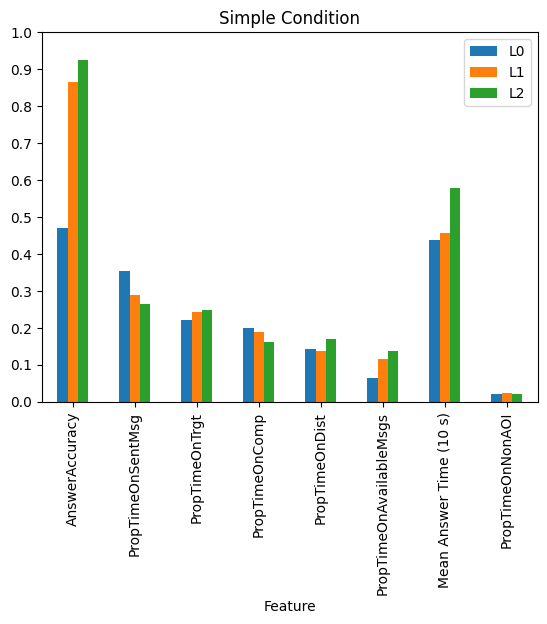
\includegraphics[width=0.46\textwidth]{images/barchart_simple.png}}{
    \vspace{0.5em} % Add padding
    \caption{Comparison of features for different labels on trials of Simple condition.}
    \label{fig:barchart_simple}
}
\ffigbox[\FBwidth]{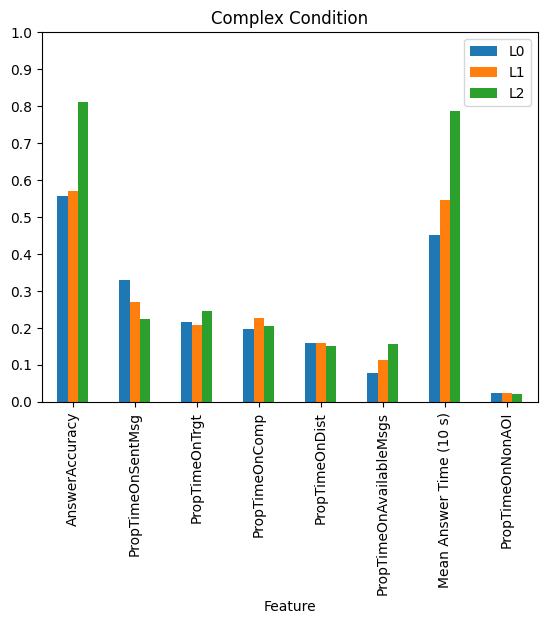
\includegraphics[width=0.46\textwidth]{images/barchart_complex.png}}{
    \vspace{0.5em} % Add padding
    \caption{Comparison of features for different labels on trials of Complex condition.}
    \label{fig:barchart_complex}
}
\end{floatrow}
\begin{floatrow}
\ffigbox[\FBwidth]{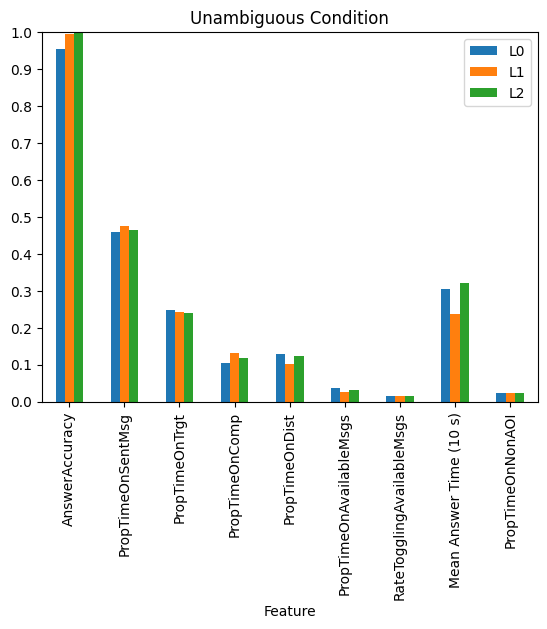
\includegraphics[width=0.48\textwidth]{images/barchart_unambiguous.png}}{
    \vspace{0.5em} % Add padding
    \caption{Comparison of features for different labels on trials of Unambiguous condition.}
    \label{fig:barchart_unambiguous}
}
\end{floatrow}
\end{figure}


\section{Predicting Accuracy via Strategies}
\label{sec:predicting_accuracy_strategies}

In order to verify that strategy labels correspond to the $L_0$, $L_1$ and $L_2$ listeners, we present the following model. The model predicts whether a trial is correctly solved based on the strategy label of the participant and some general information about the trial. Similarly to previous models we train the model only on the critical trails. 

\begin{verbatim}
    Correct ~ Condition + TrgtPos + Trial +
    StrategyLabel + MsgType + AnswerTime +
    Condition:StrategyLabel +
    (1 + Condition + TrgtPos + Trial +
    StrategyLabel + MsgType + AnswerTime | Subject)
\end{verbatim}




\begin{table}[ht]
\centering
\begin{tabular}{lrrrr}
\hline
\textbf{Predictor} & \textbf{Estimate} & \textbf{Est. Error} & \textbf{2.5\% CI} & \textbf{95\% CI} \\
\hline
Intercept                  &  1.78 & 0.15 &  1.49 &  2.08 \\
Condition1                 &  0.51 & 0.10 &  0.32 &  0.70 \\
TrgtPos2                   & -0.51 & 0.17 & -0.84 & -0.16 \\
TrgtPos3                   & -0.64 & 0.18 & -0.99 & -0.27 \\
Trial                      &  0.40 & 0.07 &  0.27 &  0.54 \\
StrategyLabel1             &  0.65 & 0.14 &  0.37 &  0.94 \\
StrategyLabel2             &  0.66 & 0.08 &  0.50 &  0.82 \\
MsgType1                   & -0.13 & 0.08 & -0.30 &  0.02 \\
AnswerTime                 & -0.06 & 0.11 & -0.26 &  0.16 \\
Condition1:StrategyLabel1  &  0.66 & 0.12 &  0.43 &  0.90 \\
Condition1:StrategyLabel2  &  0.10 & 0.06 & -0.03 &  0.23 \\
Condition1:AnswerTime      & -0.09 & 0.08 & -0.24 &  0.07 \\
\hline
\end{tabular}
\caption{Regression coefficients with estimates, errors, and 95\% credible intervals. All \texttt{Rhat} values were sufficiently close to 1, indicating convergence.}
\label{tab:cor_strtgy}
\end{table}


The general coefficients are presented in \autoref{tab:cor_strtgy}, while the strategy labels effects decomposed by condition are presented in \autoref{tab:cor_strtgy_cond}.



\begin{table}[ht]
\centering
\begin{tabular}{llrrr}
\hline
\textbf{Condition} & \textbf{StrategyLabel} & \textbf{Emmean} & \textbf{Lower HPD} & \textbf{Upper HPD} \\
\hline
complex & 0 &  0.334 & -0.0392 &  0.720 \\
simple  & 0 & -0.161 & -0.7093 &  0.379 \\
complex & 1 &  0.323 & -0.1381 &  0.780 \\
simple  & 1 &  2.443 &  1.7746 &  3.150 \\
complex & 2 &  1.997 &  1.5830 &  2.439 \\
simple  & 2 &  3.392 &  2.8847 &  3.953 \\
\hline
\end{tabular}
\caption{Estimated marginal means (emmean) with 95\% HPD intervals by Condition and Strategy Label.}
\label{tab:cor_strtgy_cond}
\end{table}

The results of \autoref{tab:cor_strtgy_cond} demonstrate that the last three rows are significant. Those are $L_1$ having positive effect for Simple condition and $L_2$ having positive effect for both critical conditions.



\section{Predicting Rate of Toggling via Strategies}
\label{sec:rate_toggling_strtg}

The model presented here predicts the rate of toggling between the available messages during correctly solved trials. The final formula for the model predicting the rate of toggling is presented below.

\begin{verbatim}
    RateTogglingAvailableMsgs ~ Condition + TrgtPos + Trial +
    StrategyLabel + Correct + MsgType + AnswerTime +
    Condition:StrategyLabel +
    (1 + Condition + TrgtPos + Trial +
    StrategyLabel + Correct + MsgType + AnswerTime | Subject)
\end{verbatim}

where \texttt{StrategyLabel} is a categorical variable that indicates the strategy label of the participant, which was derived from the annotations of the strategies that participants entered in the end of the experiment. The \texttt{Correct} variable indicates whether the trial was solved correctly or not. The model was trained using the \texttt{brms} package in R. The model was trained using the \texttt{brm} function. The resulting coefficients can be seen in \autoref{tab:model_coefficients_rate_toggling}.



\begin{table}[ht]
\centering
\caption{Regression coefficients from the model. All $\hat{R}$ values were close to 1, indicating convergence.}
\begin{tabular}{lrrrr}
\hline
\textbf{Predictor} & \textbf{Estimate} & \textbf{Est. Error} & \textbf{2.5\% CI} & \textbf{97.5\% CI} \\
\hline
Intercept                  & 0.00160 & 0.00240 & -0.00314 & 0.00631 \\
Condition1                 & 0.00027 & 0.00076 & -0.00123 & 0.00177 \\
TrgtPos2                   & -0.00121 & 0.00171 & -0.00456 & 0.00211 \\
TrgtPos3                   & -0.00063 & 0.00175 & -0.00407 & 0.00279 \\
Trial                      & 0.00151 & 0.00087 & -0.00022 & 0.00321 \\
StrategyLabel1             & 0.00558 & 0.00230 & 0.00108  & 0.01010 \\
StrategyLabel2             & 0.00317 & 0.00105 & 0.00111  & 0.00523 \\
Correct                    & 0.00061 & 0.00184 & -0.00295 & 0.00424 \\
MsgType1                   & 0.00138 & 0.00071 & -0.00001 & 0.00277 \\
AnswerTime                 & 0.01530 & 0.00199 & 0.01152  & 0.01934 \\
Condition1:StrategyLabel1  & 0.00183 & 0.00105 & -0.00023 & 0.00394 \\
Condition1:StrategyLabel2  & 0.00097 & 0.00046 & 0.00006  & 0.00189 \\
\hline
\end{tabular}
\label{tab:model_coefficients_rate_toggling}
\end{table}


The coefficients demonstrate that the rate of toggling is positively associated with the \texttt{AnswerTime} feature, which is also supported by the correlation analysis in \autoref{sec:analysis:corr}. Moreover, the general coefficients of \texttt{StrategyLabel} are significant and indicate that more skilled participants according to the labels toggle with a higher rate than less skilled ones. Furthermore, one can look at the decomposition according to condition in \autoref{tab:rate_toggling_emmeans}. The results indicate that the rate of toggling has a significant negative effect for $L_0$ listeners in Simple condition. As well as positive significant effect for $L_2$ listeners in both Simple and Complex conditions. Further supporting the idea that more skilled participants toggle more often than less skilled ones. 

\begin{table}[ht]
\centering
\begin{tabular}{l c r r r}
\hline
\textbf{Condition} & \textbf{StrategyLabel} & \textbf{Emmean} & \textbf{Lower.HPD} & \textbf{Upper.HPD} \\
complex & 0 & -0.00494 & -0.01197 &  0.00197 \\
simple  & 0 & -0.00999 & -0.01701 & -0.00308 \\
complex & 1 &  0.00259 & -0.00454 &  0.00975 \\
simple  & 1 &  0.00485 & -0.00238 &  0.01203 \\
complex & 2 &  0.00545 &  0.00061 &  0.00994 \\
simple  & 2 &  0.00984 &  0.00519 &  0.01467 \\
\hline
\end{tabular}
\caption{Estimated marginal means (emmean) with 95\% HPD intervals by condition and strategy label.}
\label{tab:rate_toggling_emmeans}
\end{table}





\section{Scanpath Analysis}
\label{sec:scanpath_analysis}
The scanpath analysis is a difficult analysis as the data itself has different lengths. This means that one cannot directly use similar models as we did for the other features. Hence, we resort to the following approach of modeling the scanpaths as Markov Models.


\subsection{Markov Model}
\label{sec:markov_model}
The Markov Model is a statistical model that describes the scanpath with a matrix of transition conditional probabilities. That is, the model describes the probability of transitioning from one area of interest to another. The approach is similar to the one used by \cite{Coutrot_2018}. The main difference is that we do not use the hidden Markov Model, as we defined the areas of interest ourselves. \autoref{fig:trans_mat} presents the transition matrices for the $L_0$, $L_1$ and $L_2$ listeners. It is important to note that due to the fact that no fixation detection was done, the diagonal elements of the matrices are very high comparing to other elements. This is expected as the participants are likely to look at the same area of interest multiple times during one fixation which is not compressed to one event. 

\begin{figure}
    \centering
    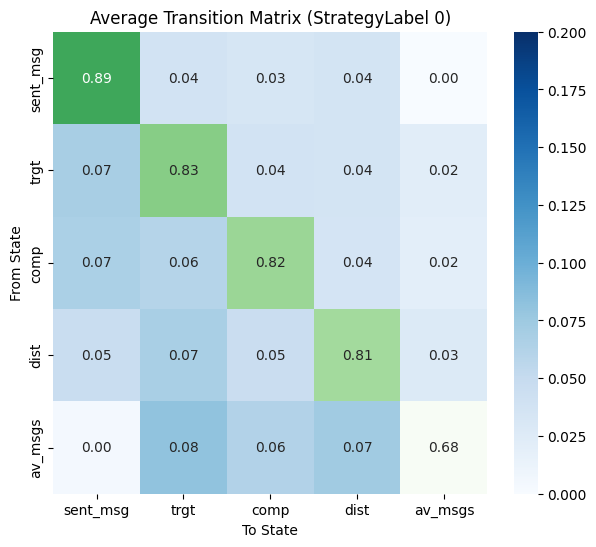
\includegraphics[width=0.3\textwidth]{images/trans_mat_l0.png}
    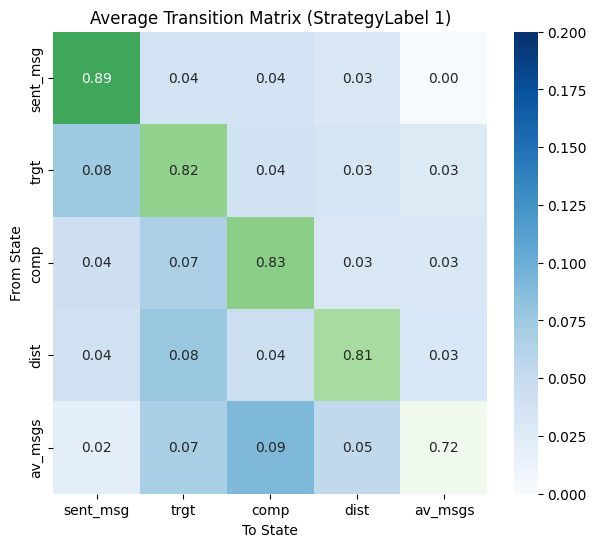
\includegraphics[width=0.3\textwidth]{images/trans_mat_l1.png}
    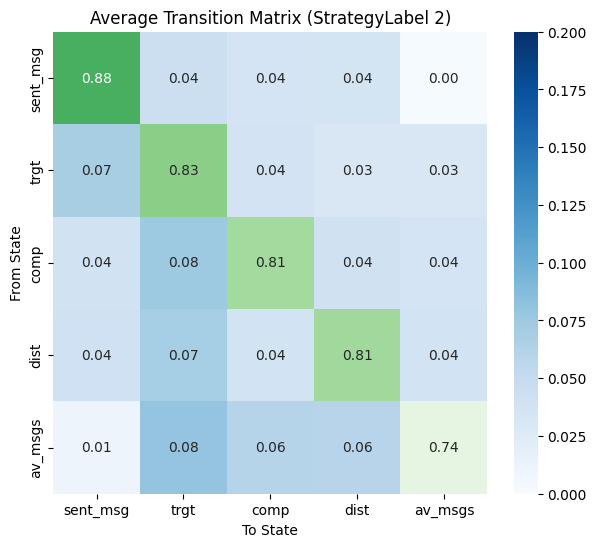
\includegraphics[width=0.3\textwidth]{images/trans_mat_l2.png}
    \caption{Average transition matrices for the $L_0$, $L_1$ and $L_2$ listeners.}
    \label{fig:trans_mat}
\end{figure}

The resulting entries of transition matrices were used as features to predict the labels of the listeners. Due to the three classes of listeners, we used tree classifiers, one for each critical condition. The trees' hyperparameters were tuned using the \texttt{GridSearchCV} function from the \texttt{sklearn} package in Python. 
In order to keep interpretability of the results, we limited the search space of max\_depth up to 4. The cross validation had 5 folds. The best mean f1 weighted score for the Simple condition amounted at 0.47 and for the Complex condition at 0.51. Further we present the visualization of the trees trained on the whole data using the best found hyperparameters in \autoref{fig:scanp_trees}. The trees were trained based on Gini impurity. It can be seen at every node indicating its purity. The top part of the node indicates the feature that was used to split the data at that node. Furthermore, the value gives us insight into the current distribution of the labels at that node. The higher the value for a certain class is the more likely the class is to be predicted at that node.

\begin{figure}
    \centering
    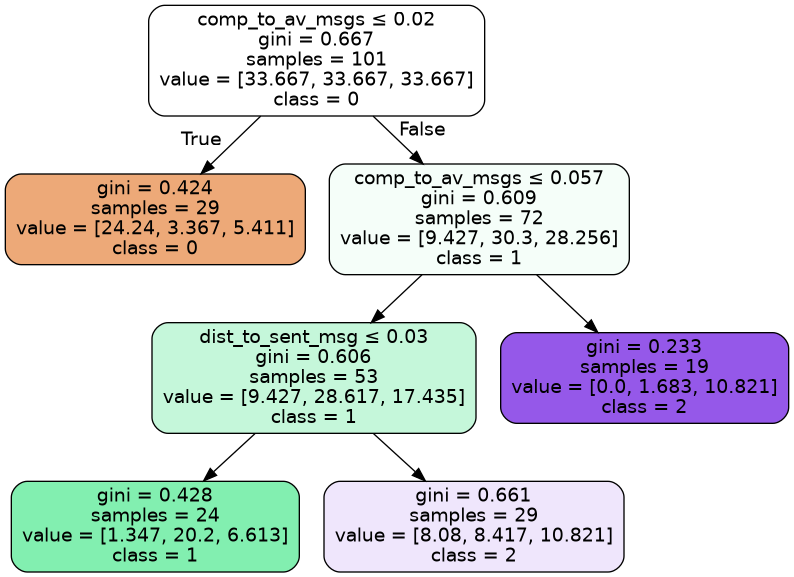
\includegraphics[width=0.45\textwidth]{images/tree_classifier_scanp_simple.png}
    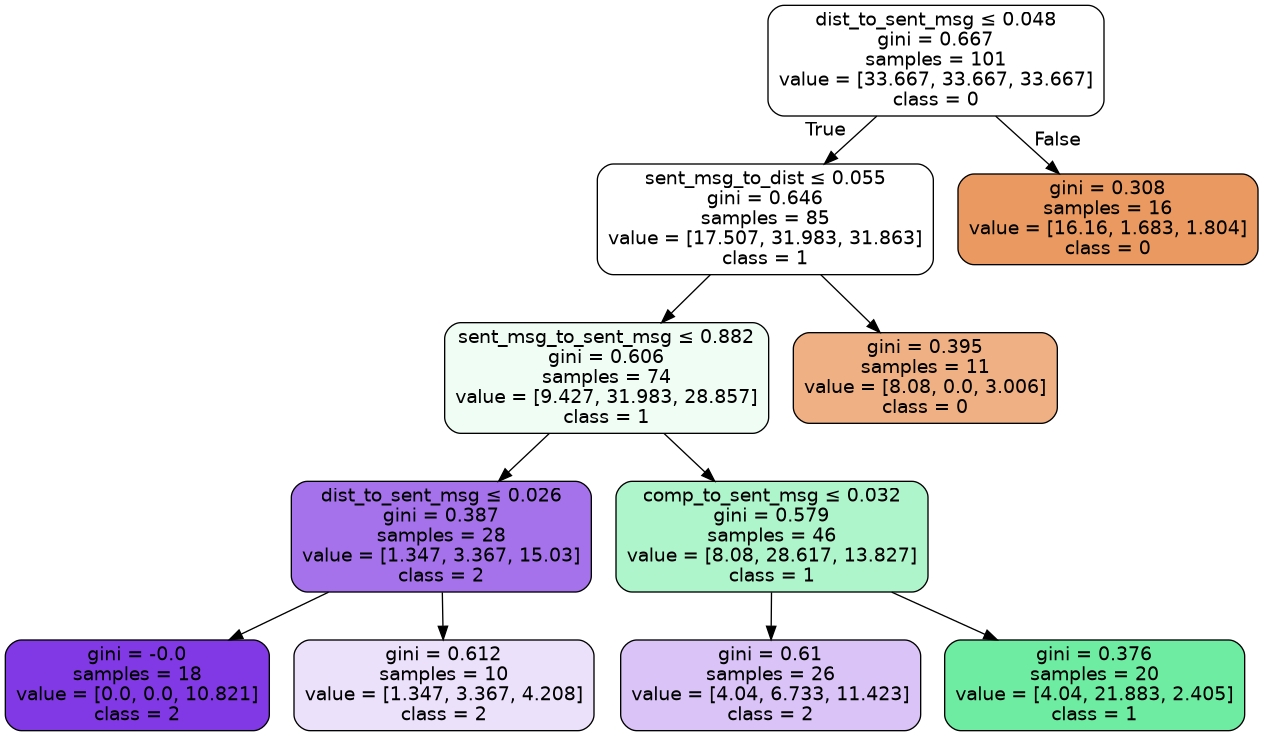
\includegraphics[width=0.45\textwidth]{images/tree_classifier_scanp_complex.png}
    \caption{Scanpath based trees for the Simple (left) and Complex (right) conditions.}
    \label{fig:scanp_trees}
\end{figure}

Even though the scores are not particularly impressive, we would like to interpret some of the splits made by the decision trees along the way. The Simple condition tree in \autoref{fig:scanp_trees} indicates that the the available messages features allow for good splits in the data, 
firstly identifying $L_0$ listeners with low \texttt{comp\_to\_av\_msgs} values. And yet another split on the same feature allows to identify $L_2$ listeners with high \texttt{comp\_to\_av\_msgs} values.

The Complex condition tree, on the other hand, involves Distractor features at the top levels. The root node splits on \texttt{dist\_to\_sent\_msg} feature, while the following node splits on \texttt{sent\_msg\_to\_dist}, low values at both splits indicate $L_0$ listeners. It is not particularly clear how the Distractor and sent message interact in this setting, however, the Distractor is clearly important for the Complex condition.


Furthermore, we compared the features derived from transition matrices to the proportional features we used in the main model. The best mean f1 weighted score for the Simple condition amounted at 0.5 and for the Complex condition at 0.56. Potentially indicating that the proportional features are more informative than the transition matrices. The visualizations of the trees trained on the proportional features can be seen in \autoref{fig:scanp_trees_prop}. 

\begin{figure}
    \centering
    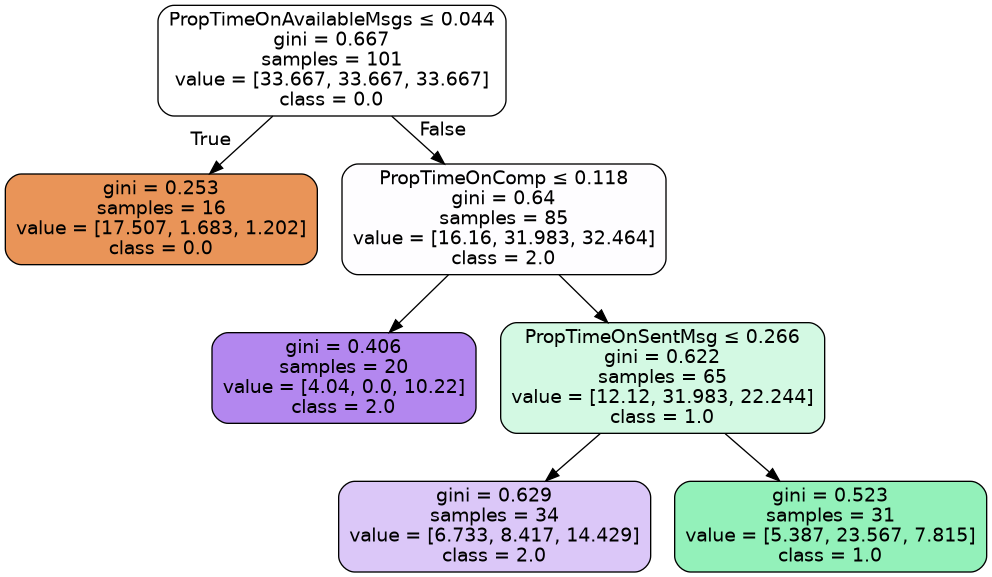
\includegraphics[width=0.45\textwidth]{images/tree_classifier_prop_simple.png}
    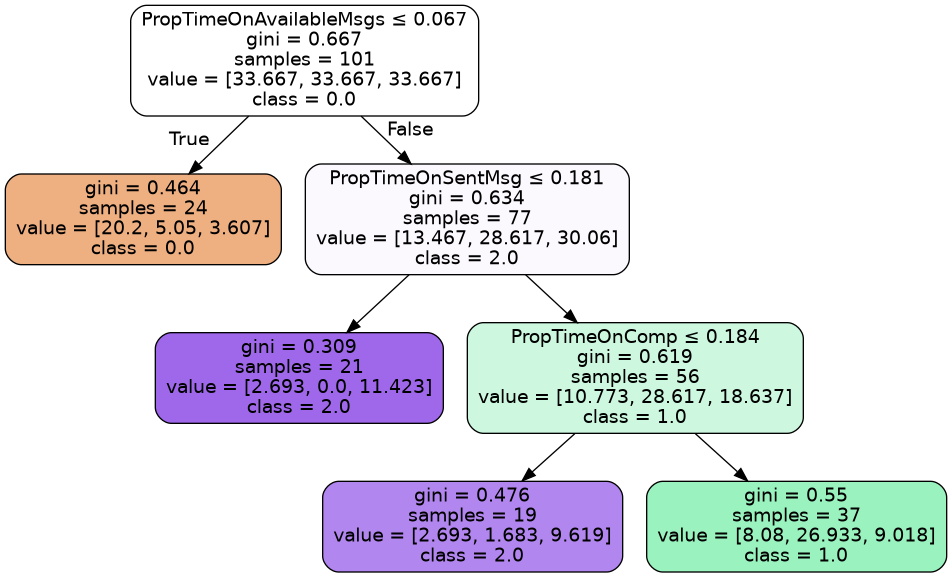
\includegraphics[width=0.45\textwidth]{images/tree_classifier_prop_complex.png}
    \caption{\texttt{PropTimeOn} based trees for the Simple (left) and Complex (right) conditions based on proportional features.}
    \label{fig:scanp_trees_prop}
\end{figure}

The trees in this case look very similar for both conditions, potentially indicating that the transition matrices were able to make a better distinguish between them. Available messages are again found to be important, in this case, for both conditions, being on the very top of the tree, their split distinguishes $L_0$ listeners from $L_1$ and $L_2$. In contrast to the scanpath based trees, the Distractor is not found to be important in this case. 




\section{ACT-R Model}
\label{sec:actr_model}
As we analyze eye-tracking data, the following paper by \TODO{add citation} presents an ACT-R model that simulates participants with different strategies. Hence, this section is dedicated to the data generated by the ACT-R model. The main goal of this section is to analyze the data generated by the ACT-R model and compare it to the data collected from the participants. The ACT-R model was trained on the same trials as the participants, it included variety of hyperparameters, mimicking the participants' behavior. The resulting coefficients for the same regression as in \autoref{sec:accuracy_model} can be seen in \autoref{tab:actr_model_coefficients}. 

\begin{table}[ht]
\centering
\begin{tabular}{lrrrr}
\hline
\textbf{Predictor} & \textbf{Estimate} & \textbf{Est. Error} & \textbf{2.5\% CI} & \textbf{95\% CI} \\
\hline
Intercept                               & 0.85 & 0.01 & 0.82  & 0.87  \\
Condition1                              & 0.23 & 0.01 & 0.22  & 0.24  \\
Trial                                  & 0.15 & 0.01 & 0.14  & 0.16  \\
PropTimeOnTrgt                         & 0.82 & 0.05 & 0.71  & 0.92  \\
PropTimeOnComp                         & 0.75 & 0.05 & 0.65  & 0.86  \\
PropTimeOnDist                         & 0.72 & 0.05 & 0.61  & 0.82  \\
PropTimeOnSentMsg                      & 6.34 & 0.29 & 5.78  & 6.90  \\
PropTimeOnAvailableMsgs               & -1.79 & 0.09 & -1.97 & -1.61 \\
RateTogglingAvailableMsgs              & 3.44 & 4.63 & -5.46 & 12.48 \\
AnswerTime                            & 1.22 & 0.03 & 1.17  & 1.27  \\
Condition1:PropTimeOnTrgt             & -0.74 & 0.05 & -0.83 & -0.65 \\
Condition1:PropTimeOnComp             & -0.83 & 0.05 & -0.93 & -0.74 \\
Condition1:PropTimeOnDist             & -0.73 & 0.05 & -0.82 & -0.64 \\
Condition1:PropTimeOnSentMsg          & -3.09 & 0.25 & -3.58 & -2.60 \\
Condition1:PropTimeOnAvailableMsgs    & 1.46 & 0.08 & 1.31  & 1.62  \\
Condition1:RateTogglingAvailableMsgs  & 1.19 & 4.65 & -7.87 & 10.22 \\
Condition1:AnswerTime                 & -0.25 & 0.02 & -0.30 & -0.21 \\
\hline
\end{tabular}
\caption{Regression coefficients with estimates, standard errors, and 95\% credible intervals. All \texttt{Rhat} values were sufficiently close to 1, indicating convergence.}
\label{tab:actr_model_coefficients}
\end{table}

The coefficients do not align with the ones from the real participants, indicating that the ACT-R model does not simulate the eye-tracking data well. The main reason for it being, overusage of the memory feature. That is, the more complex reasoning is encoded via the same eye-tracking movements. The model firstly scans each of the available messages, then each of the referents. Because the order of the referents is randomized the last fixation is one of the referents picked randomly. After the last fixation, the model performs reasoning solely relying on memory. Therefore, not simulating the real-data well. The final features therefore, result in high proportional values in one of the referents. not indicating the reasoning process well.

Due to absence of the reasoning process, we further investigate the value of \texttt{PropTimeOnAvailableMsgs} feature. We visualize the counts for each condition, strategy label and correct values. The plot can be seen in \autoref{fig:actr_prop_time_on_av_msgs}. 

\begin{figure}
    \centering
    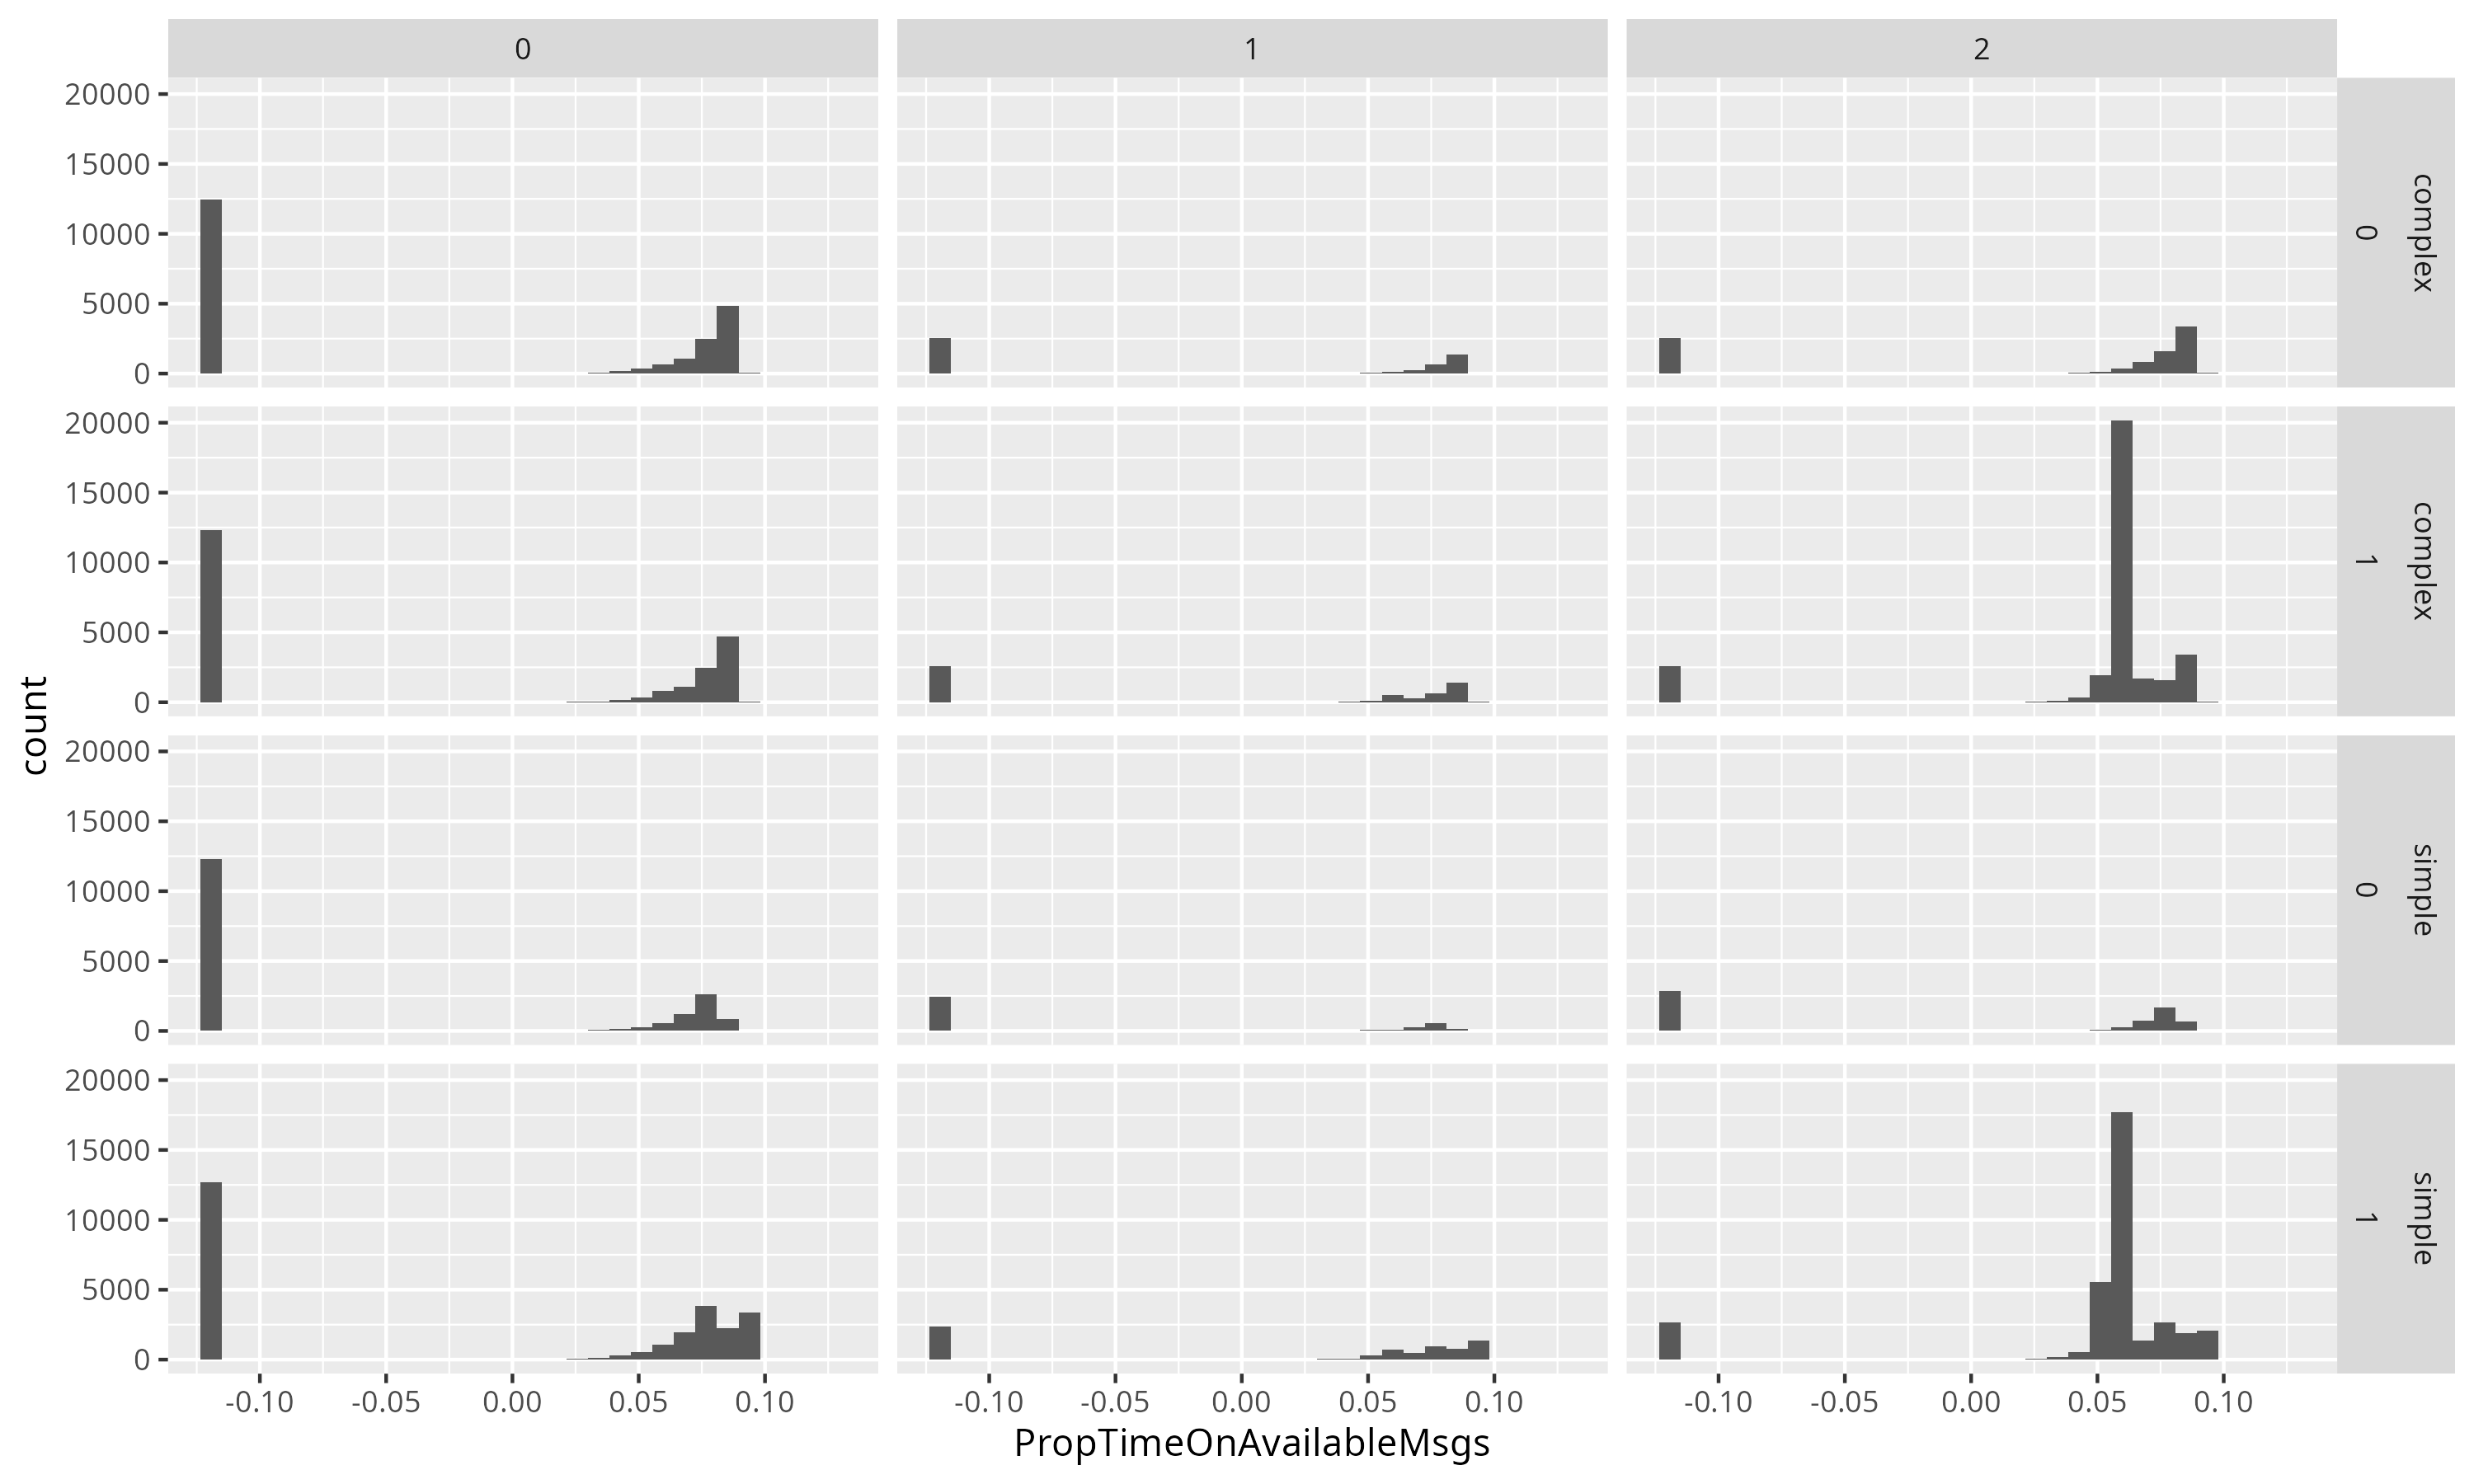
\includegraphics[width=0.8\textwidth]{images/sim_av_msgs_plot.png}
    \caption{Counts of the \texttt{PropTimeOnAvailableMsgs} feature for the ACT-R model.}
    \label{fig:actr_prop_time_on_av_msgs}
\end{figure}

\TODO{further explain the plot and the results.}